% --------------------------------------------------------------------------- %
% Poster for the ECCS 2011 Conference about Elementary Dynamic Networks.      %
% --------------------------------------------------------------------------- %
% Created with Brian Amberg's LaTeX Poster Template. Please refer for the     %
% attached README.md file for the details how to compile with `pdflatex`.     %
% --------------------------------------------------------------------------- %
% $LastChangedDate:: 2011-09-11 10:57:12 +0200 (V, 11 szept. 2011)          $ %
% $LastChangedRevision:: 128                                                $ %
% $LastChangedBy:: rlegendi                                                 $ %
% $Id:: poster.tex 128 2011-09-11 08:57:12Z rlegendi                        $ %
% --------------------------------------------------------------------------- %
\documentclass[a0paper,portrait]{baposter}

\usepackage{relsize}		% For \smaller
\usepackage{url}			% For \url
% \usepackage{epstopdf}	% Included EPS files automatically converted to PDF to include with pdflatex

%%% Global Settings %%%%%%%%%%%%%%%%%%%%%%%%%%%%%%%%%%%%%%%%%%%%%%%%%%%%%%%%%%%

\graphicspath{{pix/}}	% Root directory of the pictures 
% \tracingstats=2			% Enabled LaTeX logging with conditionals

%%% Color Definitions %%%%%%%%%%%%%%%%%%%%%%%%%%%%%%%%%%%%%%%%%%%%%%%%%%%%%%%%%

\definecolor{bordercol}{RGB}{40,40,40}
\definecolor{headercol1}{RGB}{186,215,230}
\definecolor{headercol2}{RGB}{80,80,80}
\definecolor{headerfontcol}{RGB}{0,0,0}
\definecolor{boxcolor}{RGB}{186,215,230}

%%%%%%%%%%%%%%%%%%%%%%%%%%%%%%%%%%%%%%%%%%%%%%%%%%%%%%%%%%%%%%%%%%%%%%%%%%%%%%%%
%%% Utility functions %%%%%%%%%%%%%%%%%%%%%%%%%%%%%%%%%%%%%%%%%%%%%%%%%%%%%%%%%%

%%% Save space in lists. Use this after the opening of the list %%%%%%%%%%%%%%%%
\newcommand{\compresslist}{
	\setlength{\itemsep}{1pt}
	\setlength{\parskip}{0pt}
	\setlength{\parsep}{0pt}
}

%%%%%%%%%%%%%%%%%%%%%%%%%%%%%%%%%%%%%%%%%%%%%%%%%%%%%%%%%%%%%%%%%%%%%%%%%%%%%%%
%%% Document Start %%%%%%%%%%%%%%%%%%%%%%%%%%%%%%%%%%%%%%%%%%%%%%%%%%%%%%%%%%%%
%%%%%%%%%%%%%%%%%%%%%%%%%%%%%%%%%%%%%%%%%%%%%%%%%%%%%%%%%%%%%%%%%%%%%%%%%%%%%%%

\begin{document}
\typeout{Poster rendering started}

%%% Setting Background Image %%%%%%%%%%%%%%%%%%%%%%%%%%%%%%%%%%%%%%%%%%%%%%%%%%
\background{
	\begin{tikzpicture}[remember picture,overlay]%
	\draw (current page.north west)+(-2em,2em) node[anchor=north west]
	{\includegraphics[height=1.1\textheight]{background}};
	\end{tikzpicture}
}

%%% General Poster Settings %%%%%%%%%%%%%%%%%%%%%%%%%%%%%%%%%%%%%%%%%%%%%%%%%%%
%%%%%% Eye Catcher, Title, Authors and University Images %%%%%%%%%%%%%%%%%%%%%%
\begin{poster}{
	grid=false,
	% Option is left on true though the eyecatcher is not used. The reason is
	% that we have a bit nicer looking title and author formatting in the headercol
	% this way
	%eyecatcher=false, 
	borderColor=bordercol,
	headerColorOne=headercol1,
	headerColorTwo=headercol2,
	headerFontColor=headerfontcol,
	% Only simple background color used, no shading, so boxColorTwo isn't necessary
	boxColorOne=boxcolor,
	headershape=roundedright,
	headerfont=\Large\sf\bf,
	textborder=rectangle,
	background=user,
	headerborder=open,
  boxshade=plain
}
%%% Eye Cacther %%%%%%%%%%%%%%%%%%%%%%%%%%%%%%%%%%%%%%%%%%%%%%%%%%%%%%%%%%%%%%%
{
	Eye Catcher, empty if option eyecatcher=false - unused
}
%%% Title %%%%%%%%%%%%%%%%%%%%%%%%%%%%%%%%%%%%%%%%%%%%%%%%%%%%%%%%%%%%%%%%%%%%%
{\sf\bf
	Complexity Science Approach To Atrial Fibrillation
}
%%% Authors %%%%%%%%%%%%%%%%%%%%%%%%%%%%%%%%%%%%%%%%%%%%%%%%%%%%%%%%%%%%%%%%%%%
{
	\vspace{1em} Tigany Zarrouk \& Mattia Gaggi\\
	%{\smaller legendi@inf.elte.hu, lgulyas@colbud.hu, gkampis@colbud.hu}
}
%%% Logo %%%%%%%%%%%%%%%%%%%%%%%%%%%%%%%%%%%%%%%%%%%%%%%%%%%%%%%%%%%%%%%%%%%%%%
%{
% The logos are compressed a bit into a simple box to make them smaller on the result
% (Wasn't able to find any bigger of them.)
%\setlength\fboxsep{0pt}
%\setlength\fboxrule{0.5pt}
%	\fbox{
%		\begin{minipage}{14em}
%			\includegraphics[width=10em,height=4em]{colbud_logo}
%			\includegraphics[width=4em,height=4em]{elte_logo} \\
%			\includegraphics[width=10em,height=4em]{dynanets_logo}%
%			\includegraphics[width=4em,height=4em]{aitia_logo}
%		\end{minipage}
%	}
%}

\headerbox{Problem}{name=problem,column=0,row=0}{
Modelling Atrial Fibrillation (AF) to ascertain its causes accurately, allowing for effective treatment, has been extensively studied over the past few decades. It is the largest cause of strokes linked with cardiac arrhythmia in aging populations and is due to impaired contractility of the atria in the heart, leading to blood clot formation. Action potential propagation, mediated by ionic species, are seen to be irregular in AF, which causes some atrial myocytes to contract at 300+ times per minute, much faster than healthy hearts which contract at 60-100 times per minute.


This beating is regulated by the sinoatrial node which initiates action potentials that propagate through myocytes, causing contractions. Altered refractory period and conduction speed of signals has been seen to promote AF in various models and is caused physically by the fibrosis of cells, reducing the coupling of electrical signals transversally to some myocytes; giving rise to reentry circuits. The most prominent reentry model, the spiral wave model, has been seen to more closely follow clinical and experimental observations than other models of wavefront action. Cellular automata modelling paves the way for large scale simulations of tissue in the heart without the need to solve differential equations, which can be computationally costly.
%\begin{figure}
%\caption[short title]{Diagram showing a spiral wave reentry circuit. (a), a normal wavefront in the heart. (b) spiral wave, which simulates tachycardia, as can be seen by multiple propagating wavefronts in a small area. (c), turbulent activity due to break up of spiral wave giving rise to fibrillation \cite{Alonso}}
%\centering
%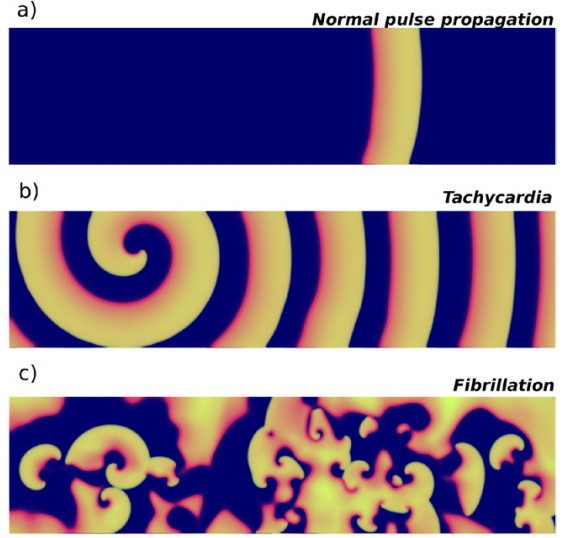
\includegraphics[width = 0.5\textwidth]{spiralbreak2tachy}
%\end{figure}
}

\headerbox{Basic Concepts}{name=definitions,column=0,below=problem}{
Originally, a model devised by Christensen \emph(et al.), modelled atrial tissue of the heart using a 200x200 lattice of cells, whereby cells along rows were fully connected to each other---replicating myocardial fibres---and cells in columns were connected to each other with a probability $\nu$  Furthermore, a proportion of the cells were deigned to be dysfunctional with a probability $\delta$ which had a probability $\epsilon$ of not being excited by an adjacent excited cell connected to it: this simulated the effects of fibrosis of cells in the heart. Tachycardia was simulated by using a period of 220 timesteps for a heartbeat and cells, once excited, had a refractory period of 50 timesteps. As can be seen in the figures below, chaotic, fibrillatory activity arised spontaneously from the model. 
}

\headerbox{Models}{name=models,column=0,below=definitions}{
\textbf{ER1} $G_0$ is a random graph. Add each non-existing edge with $p_A$, delete each existing edge with $p_D$ probability. \\
\textbf{ER2} $G_0$ is a random graph. Add $k_A$ uniformly selected random new edges and delete $k_D$ existing edges. \\
\textbf{ER3} $G_0$ is a random graph. Rewire $k_{RW}$ edges. \\
%\textbf{SPA} (\emph{Snapshot preferential}) $G_0$ is a scale free network. Add $k_A$ edges from a random node with preferential attachment based on the snapshot network. Delete $k_D$ existing edges. \\
%\textbf{CPA} (\emph{Cumulative preferential}) $G_0$ is a scale free network. Add $k_A$ edges from a random node with preferential attachment based on the cumulative network. Delete $k_D$ existing edges.
}

\headerbox{References}{name=references,column=0,below=models}{
\smaller													% Make the whole text smaller
\vspace{-0.4em} 										% Save some space at the beginning
\bibliographystyle{plain}							% Use plain style
\renewcommand{\section}[2]{\vskip 0.05em}		% Omit "References" title
\begin{thebibliography}{1}							% Simple bibliography with widest label of 1

\end{thebibliography}
}

\headerbox{Acknowledgements}{name=acknowledgements,column=0,below=references, above=bottom}{
\smaller						% Make the whole text smaller
\vspace{-0.4em}			% Save some space at the beginning
This research was partially supported by the Hungarian Government (KMOP-1.1.2-08/1-2008-0002 ) and the European Union's Seventh Framework Programme: DynaNets, FET-Open project no. FET-233847 (\url{http://www.dynanets.org}). The supports are gratefully acknowledged.
} 

\headerbox{Dynamic Networks are Sensitive to Aggregation}{name=density,span=2,column=1,row=0}{
Network characteristics are extremely sensitive to minor changes in aggregation length. In our previous work \cite{prevWork1} \cite{prevWork2}, we studied the cumulative properties of Elementary Dynamic Network models over the complete time period (i.e., until they reach the stable point of a full network). Here we focus on the more realistc domain of sparse (cumulative) networks. We find that even when snapshot networks are stationary, \textbf{important network characteristics}  (average path lenght, clustering, betwenness centrality) \textbf{are extremely sensitive to aggregation} (window length). 

%\includegraphics[angle=-90,width=0.98\linewidth]{PA_and_ER_Models_statisticalMeasures}

}

\headerbox{Degree Distribution Radically Changes}
{name=degreeDistribution,span=2,column=1,below=density,above=bottom}{
Degree distributions are exceptionally sensitive to the length of the aggregation window. \textbf{The same dynamic network may produce a normal, lognormal or even power law distribution for different aggregation lenghts.} The digree distribution of the snapshot and cumulative network is inherently different. The following surfaces show the CPA model until it approaches the complete network.
\vspace{-0.2em}
\begin{center}
%	\includegraphics[angle=-90,width=0.49\linewidth]{CPA_3d_snapshot}
%	\includegraphics[angle=-90,width=0.49\linewidth]{CPA_3d_cumulative}
\end{center}
\vspace{-0.2em}
Taking slices of the cumulative 3D charts shows us how the degree distribution changes. The log-log charts below show the progression of these changes as the aggregation window gets larger.
\vspace{-0.2em}
\begin{center}
%	\includegraphics[angle=-90,width=0.49\linewidth]{ER1_cumulativeDegrees}
%	\includegraphics[angle=-90,width=0.49\linewidth]{CPA_cumulativeDegrees}
\end{center}
}

\end{poster}
\end{document}
